% Created 2026-05-07 qui 15:55
% Intended LaTeX compiler: pdflatex
\documentclass[11pt]{article}
\usepackage[utf8]{inputenc}
\usepackage[T1]{fontenc}
\usepackage{graphicx}
\usepackage{longtable}
\usepackage{wrapfig}
\usepackage{rotating}
\usepackage[normalem]{ulem}
\usepackage{amsmath}
\usepackage{amssymb}
\usepackage{capt-of}
\usepackage{hyperref}
\author{Wagner com ajuda do Gemini CLI}
\date{\today}
\title{Resolucao do Exercicio 1 - Estatistica Multivariada}
\hypersetup{
 pdfauthor={Wagner com ajuda do Gemini CLI},
 pdftitle={Resolucao do Exercicio 1 - Estatistica Multivariada},
 pdfkeywords={},
 pdfsubject={},
 pdfcreator={Emacs 30.2 (Org mode 9.7.11)}, 
 pdflang={English}}
\begin{document}

\maketitle
\setcounter{tocdepth}{2}
\tableofcontents

\section{Introducao}
\label{sec:orgf01a873}
Este documento apresenta a resolucao da lista 1 de exercicios do nosso
curso de introducao a analise estatística multivariada

Todos os scripts estao localizados na pasta \texttt{src/}.

Para mais detalhes tudo que foi tealizado inclusive notas de estudos
pode ser acessados em
\url{https://github.com/wagnermarques/curso\_estatistica\_multivariada}


O código que produziu estes restulados abaixo se encontram neste mesmo
repositório na pasta exercícios/exercicios\textsubscript{1}/src


obrigado
\section{Exercicio 1: Analise de Dados Binarios (Presenca-Ausencia)}
\label{sec:orge296569}
O objetivo deste exercicio e analisar a similaridade entre 8 especies com base em dados binarios utilizando diferentes coeficientes.
\subsection{Codigo de Carregamento e Processamento}
\label{sec:orgec608c0}
Os dados sao carregados de um arquivo CSV e processados para calcular as matrizes de distancia de Sorensen-Dice e Simple Matching.

\begin{verbatim}
import ex1_1_read_data_from_csv
import ex1_2_clustering_binario
from scipy.spatial.distance import squareform
import pandas as pd

# 1 read data from csv
df = ex1_1_read_data_from_csv.read_data()

print("--- Primeiras 10 linhas do dataframe ---")
print(df.head(10))

# 3 calcula matriz de distancias usando coeficiente Sorensen-Dice e Simple Matching
X = df.iloc[:, 1:].values
species = df.iloc[:, 0].values


##################################################
# criando e observando as matrizes de distancias #
##################################################
dist_dice = ex1_2_clustering_binario.calcular_matriz_distancias(X, metric='dice')
dist_sm = ex1_2_clustering_binario.calcular_matriz_distancias(X, metric='matching')

# Converter para formato quadrado para visualizacao
# isso porque sem essa conversao as mtz estao no formato otimizado o ndarry
df_dist_dice = pd.DataFrame(squareform(dist_dice), index=species, columns=species)
df_dist_sm = pd.DataFrame(squareform(dist_sm), index=species, columns=species)


print("\n--- Matriz de Distancia (Sorensen-Dice) ---")
print(df_dist_dice.round(3))

print("\n--- Matriz de Distancia (Simple Matching) ---")
print(df_dist_sm.round(3))

# 4 analyze the data using clustering_binario module (gera os dendrogramas)
print("\n--- Gerando Dendrogramas ---")
ex1_2_clustering_binario.plot_dendrogram(dist_dice, species, 'dice', 'Dendrograma - Sorensen-Dice', 'dendrograma_sorensen_dice.png')
ex1_2_clustering_binario.plot_dendrogram(dist_sm, species, 'matching', 'Dendrograma - Simple Matching', 'dendrograma_simple_matching.png')

# 5 Atribuindo grupos (exemplo de corte)
print("\n--- Atribuicao de Grupos (Exemplos) ---")

# Exemplo 1: Cortar o dendrograma Sorensen-Dice para obter 3 grupos
df_grupos_dice = ex1_2_clustering_binario.atribuir_grupos(dist_dice, species, t=3, criterion='maxclust')
print("\nGrupos (Sorensen-Dice, k=3):")
print(df_grupos_dice)

# Exemplo 2: Cortar o dendrograma Simple Matching na altura 0.4
df_grupos_sm = ex1_2_clustering_binario.atribuir_grupos(dist_sm, species, t=0.4, criterion='distance')
print("\nGrupos (Simple Matching, h=0.4):")
print(df_grupos_sm)
\end{verbatim}
\captionof{figure}{Script de Analise Binaria}
\subsection{Resultados: Dendrogramas}
\label{sec:org35ad108}
Os dendrogramas abaixo mostram como as especies se agrupam de acordo com cada metrica de distancia.

\begin{figure}[htbp]
\centering
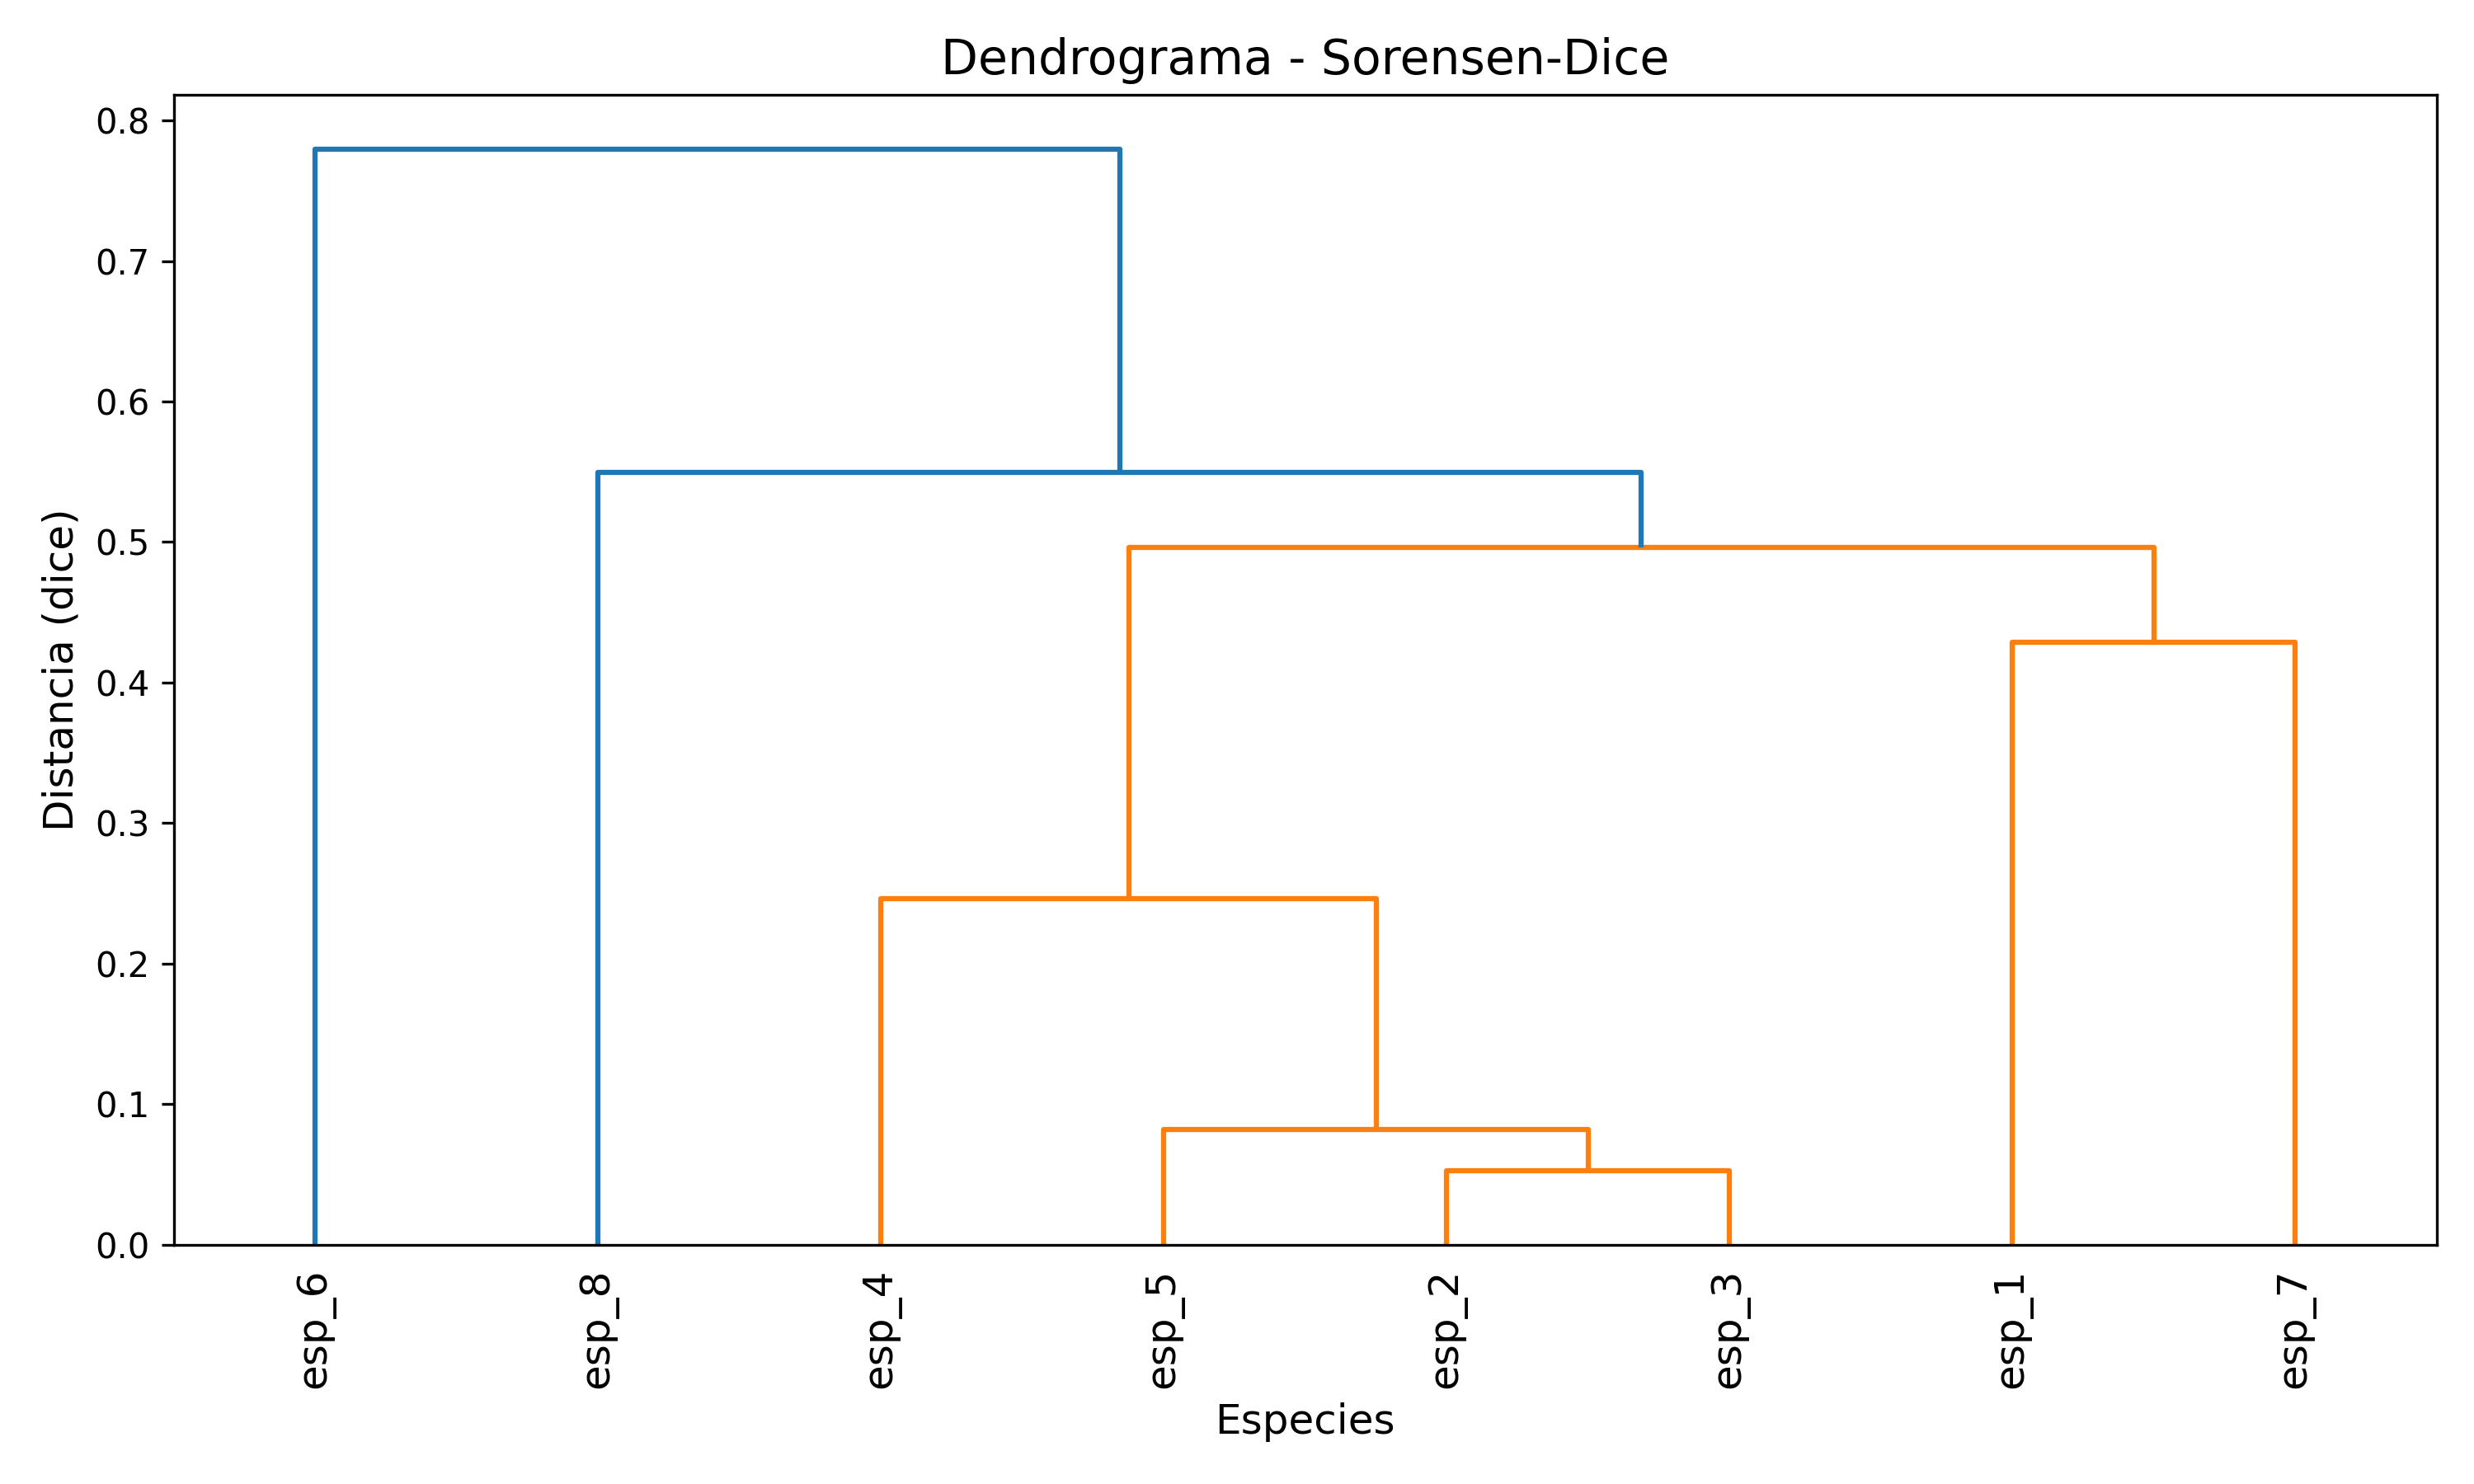
\includegraphics[width=.9\linewidth]{figures/dendrograma_sorensen_dice.png}
\caption{\label{fig:orge863e3b}Dendrograma utilizando distancia Sorensen-Dice}
\end{figure}

\begin{figure}[htbp]
\centering
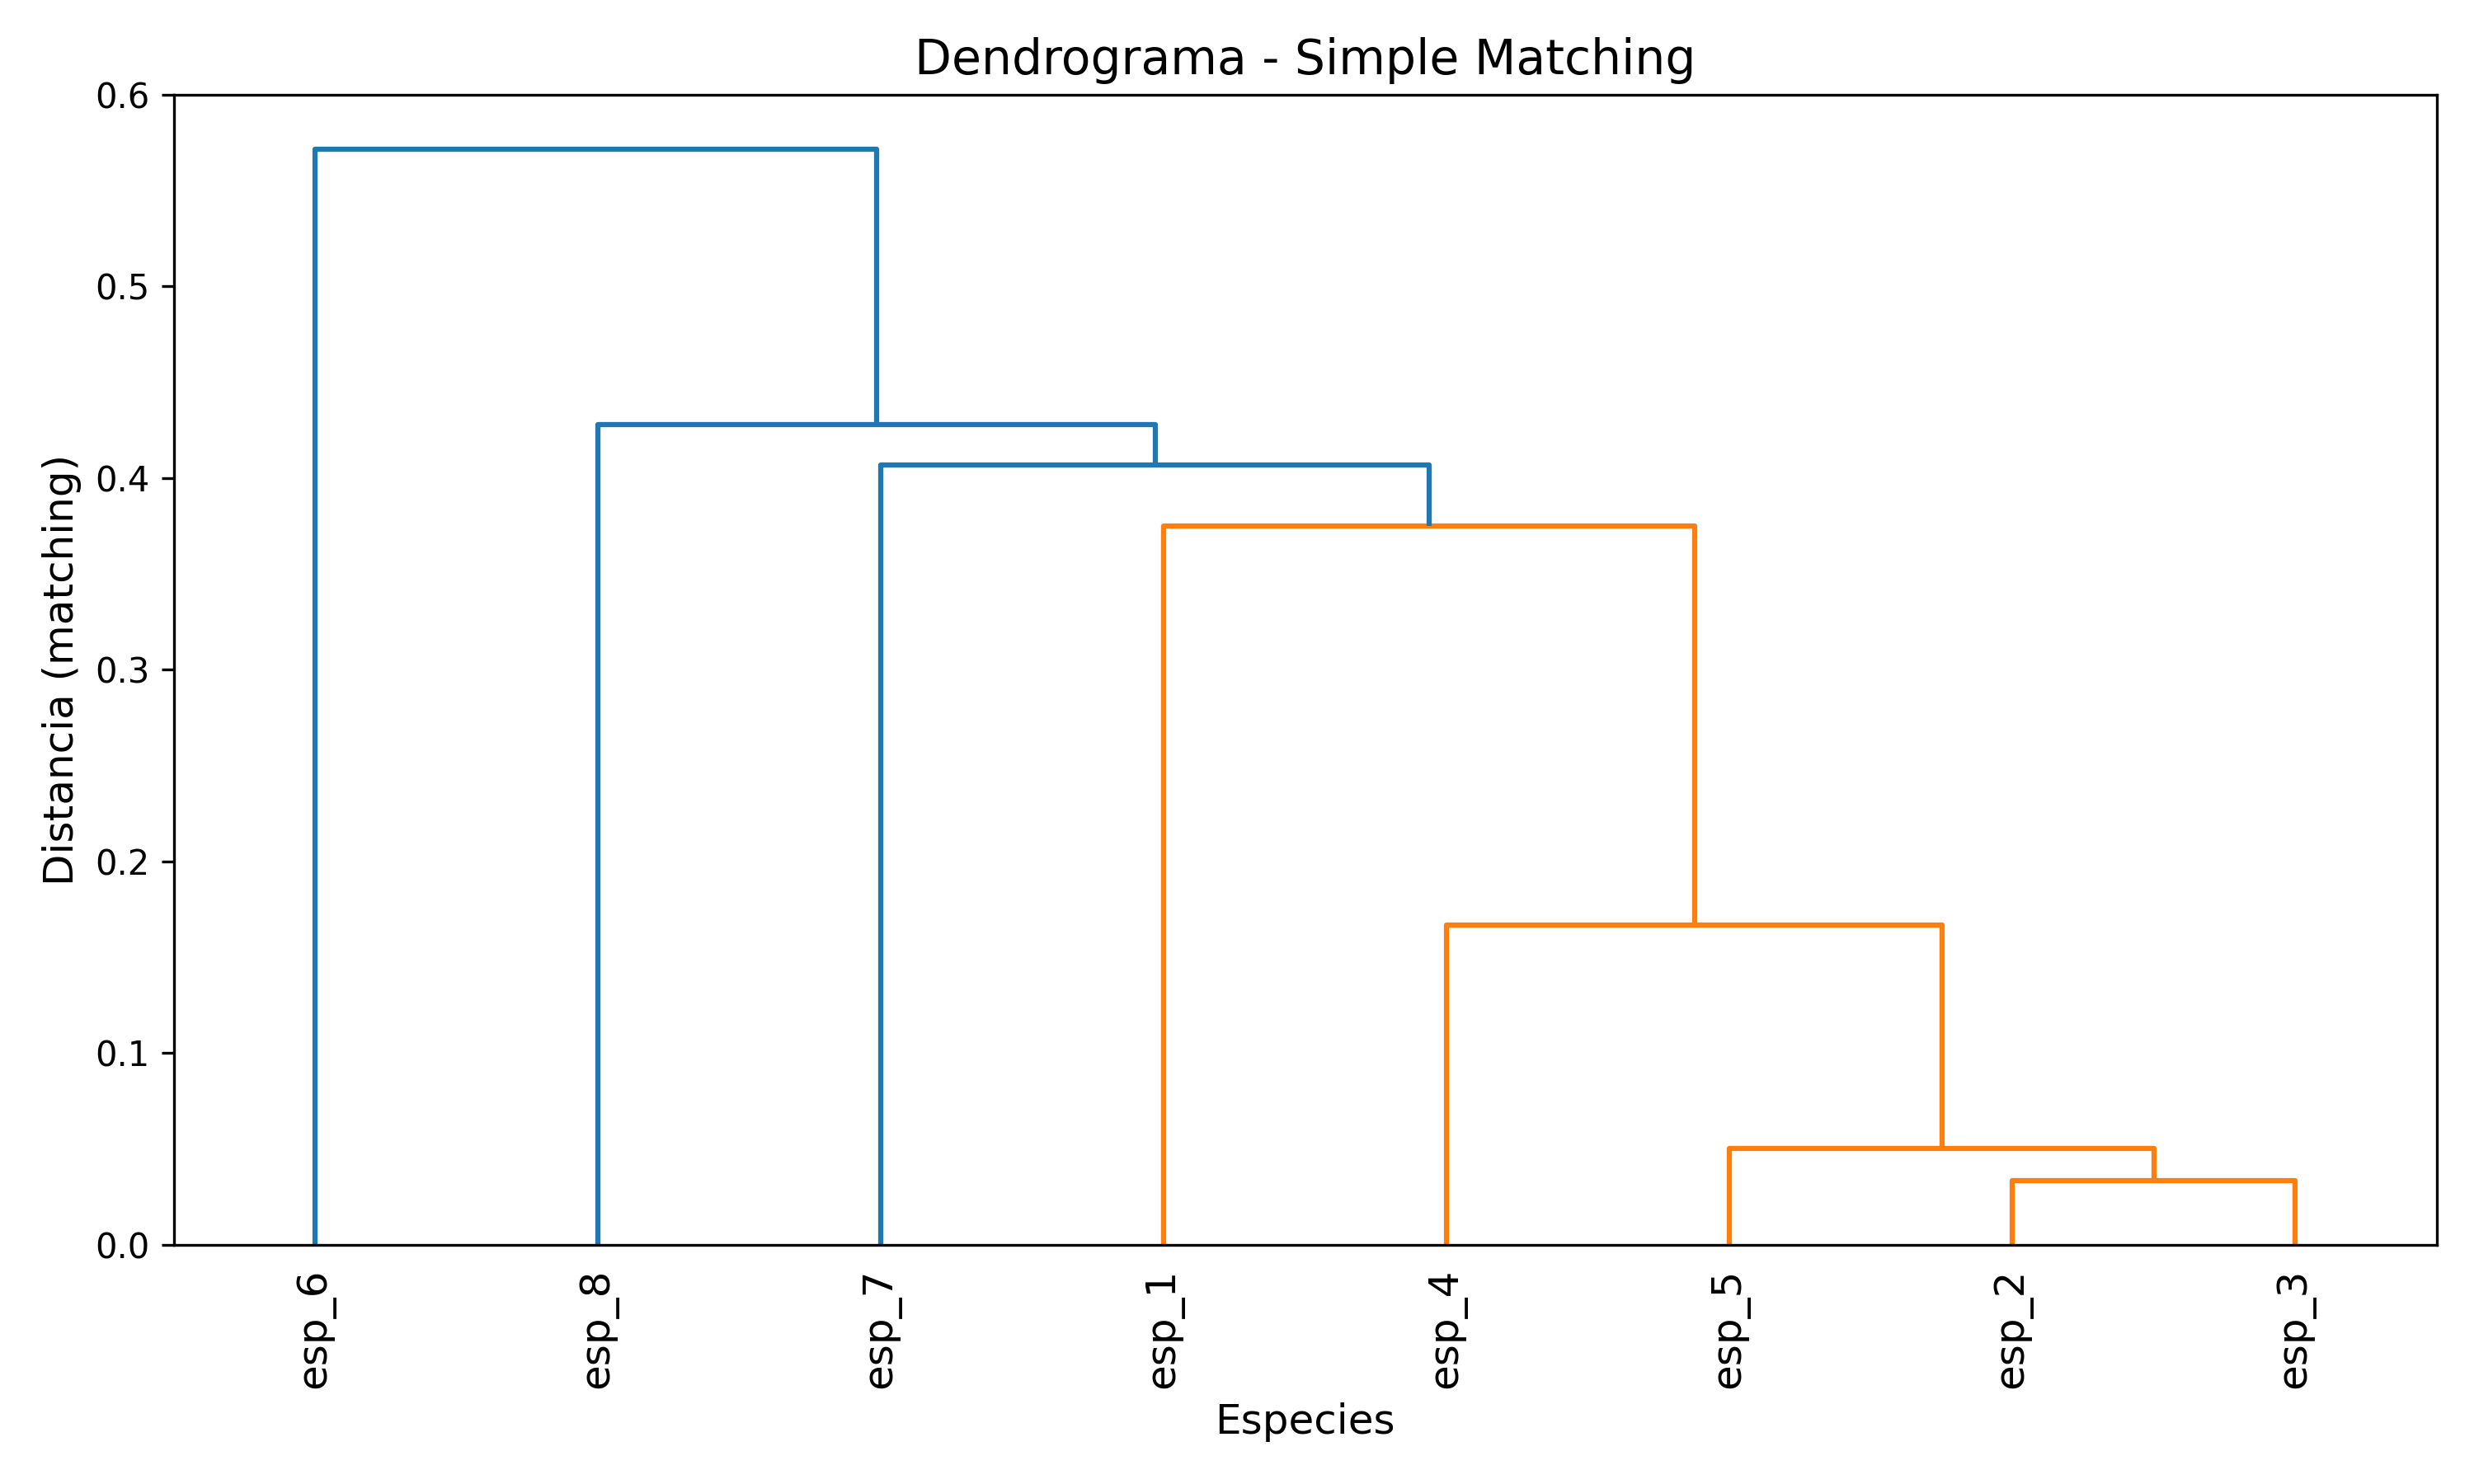
\includegraphics[width=.9\linewidth]{figures/dendrograma_simple_matching.png}
\caption{\label{fig:org79eb2a0}Dendrograma utilizando distancia Simple Matching}
\end{figure}
\section{Exercicio 2: Agrupamento K-means no Dataset IRIS}
\label{sec:org050672c}
Neste exercicio, exploramos o algoritmo K-means para agrupar flores do dataset IRIS e validamos a qualidade dos grupos formados.
\subsection{Abordagem 1: Metodo do Cotovelo (Elbow Method)}
\label{sec:org8d7e3ee}
Esta abordagem foca em encontrar o numero otimo de grupos (k) analisando a variacao da soma dos quadrados intra-cluster (WCSS).

\begin{verbatim}
import ex2_1_load_iris
import ex2_2_clustering_iris
import pandas as pd
import numpy as np
from sklearn.preprocessing import StandardScaler

# 1. Leitura dos dados
df = ex2_1_load_iris.load_iris_data()

# 2. Mostrar as primeiras 10 linhas
print("--- Primeiras 10 linhas do dataset IRIS ---")
print(df.head(10))

# 3. Padronizacao (Escalonamento)
# Selecionamos as colunas numericas (SEPALLEN, SEPALWID, PETALLEN, PETALWID)
variaveis_list = ['SEPALLEN', 'SEPALWID', 'PETALLEN', 'PETALWID']
mtz_vlrs = df[variaveis_list].values
species = df['specie'].values

scaler = StandardScaler()
mtz_vlrs_padrozinados = scaler.fit_transform(mtz_vlrs)

print("\nDados padronizados (primeiras 5 linhas):")
print(mtz_vlrs_padrozinados[:5])

# 4. Metodo do Cotovelo (Elbow Method)
print("\n--- Analise do Numero Otimo de Grupos (Metodo do Cotovelo) ---")
ex2_2_clustering_iris.plot_elbow_method(
    mtz_vlrs_padrozinados, 
    max_k=10, 
    filename='kmeans_elbow_iris.png'
)

# 5. Executar K-means
# Vamos utilizar k=3 pois sabemos que existem 3 especies no dataset IRIS
k_ideal = 3
print(f"\n--- Executando K-means (k={k_ideal}) ---")
df_grupos, kmeans_model = ex2_2_clustering_iris.executar_kmeans(
    mtz_vlrs_padrozinados, 
    species, 
    n_clusters=k_ideal
)

# Adicionando a informacao do grupo ao DataFrame original
df['Grupo'] = df_grupos['Grupo']

# 6. Mostrar resultados
print("\n--- Dados Originais com Atribuicao de Grupos (K-means) ---")
print(df.head(10))


# Verificar a contagem em cada grupo
print("\nContagem por grupo:")
print(df_grupos['Grupo'].value_counts())

# Comparar com as especies originais (Crosstab)
print("\n--- Cruzamento: Especie Original vs Grupo K-means ---")
print(pd.crosstab(df['specie'], df['Grupo']))

# 7. Visualizacao dos clusters
print("\n--- Gerando Grafico de Dispersao dos Clusters ---")
ex2_2_clustering_iris.plot_kmeans_clusters(
    mtz_vlrs_padrozinados, 
    df_grupos['Grupo'].values, 
    kmeans_model.cluster_centers_,
    filename='kmeans_scatter_iris.png'
)

# 8. Analise Univariada (ANOVA) - Verificando a qualidade dos grupos
import statsmodels.api as sm
from statsmodels.formula.api import ols

print("\n--- Analise de Variancia (ANOVA) por Variavel ---")
print("H0: Nao ha diferenca entre as medias dos grupos")
print("H1: Ha pelo menos uma diferenca entre as medias")

for var in variaveis_list:
    formula = f"{var} ~ C(Grupo)"
    model = ols(formula, data=df).fit()
    anova_table = sm.stats.anova_lm(model, typ=2)
    
    # Acessando os valores usando o nome da linha 'C(Grupo)'
    p_valor = anova_table.at['C(Grupo)', 'PR(>F)']
    f_stat = anova_table.at['C(Grupo)', 'F']
    
    print(f"\nVariavel: {var}")
    print(f"F-statistic: {f_stat:.4f}")
    print(f"p-valor: {p_valor:.4e}")
    
    if p_valor < 0.05:
        print("Resultado: Significativo (Existem diferencas entre os grupos)")
    else:
        print("Resultado: Nao significativo (Nao ha diferencas claras)")

# 9. Analise Multivariada de Variancia (MANOVA)
from statsmodels.multivariate.manova import MANOVA

print("\n--- Analise Multivariada de Variancia (MANOVA) ---")
print("H0: Os vetores de medias dos grupos sao iguais")
print("H1: Pelo menos um vetor de media e diferente")

# Criando a formula para todas as variaveis dependentes
formula_manova = " + ".join(variaveis_list) + " ~ C(Grupo)"
manova = MANOVA.from_formula(formula_manova, data=df)

# Exibindo os resultados (Wilks' lambda, Pillai's trace, etc)
print(manova.mv_test())
\end{verbatim}
\captionof{figure}{Script K-means com Metodo do Cotovelo}
\subsubsection{Graficos de Validacao do Numero de Grupos}
\label{sec:orgc1595b1}
\begin{figure}[htbp]
\centering
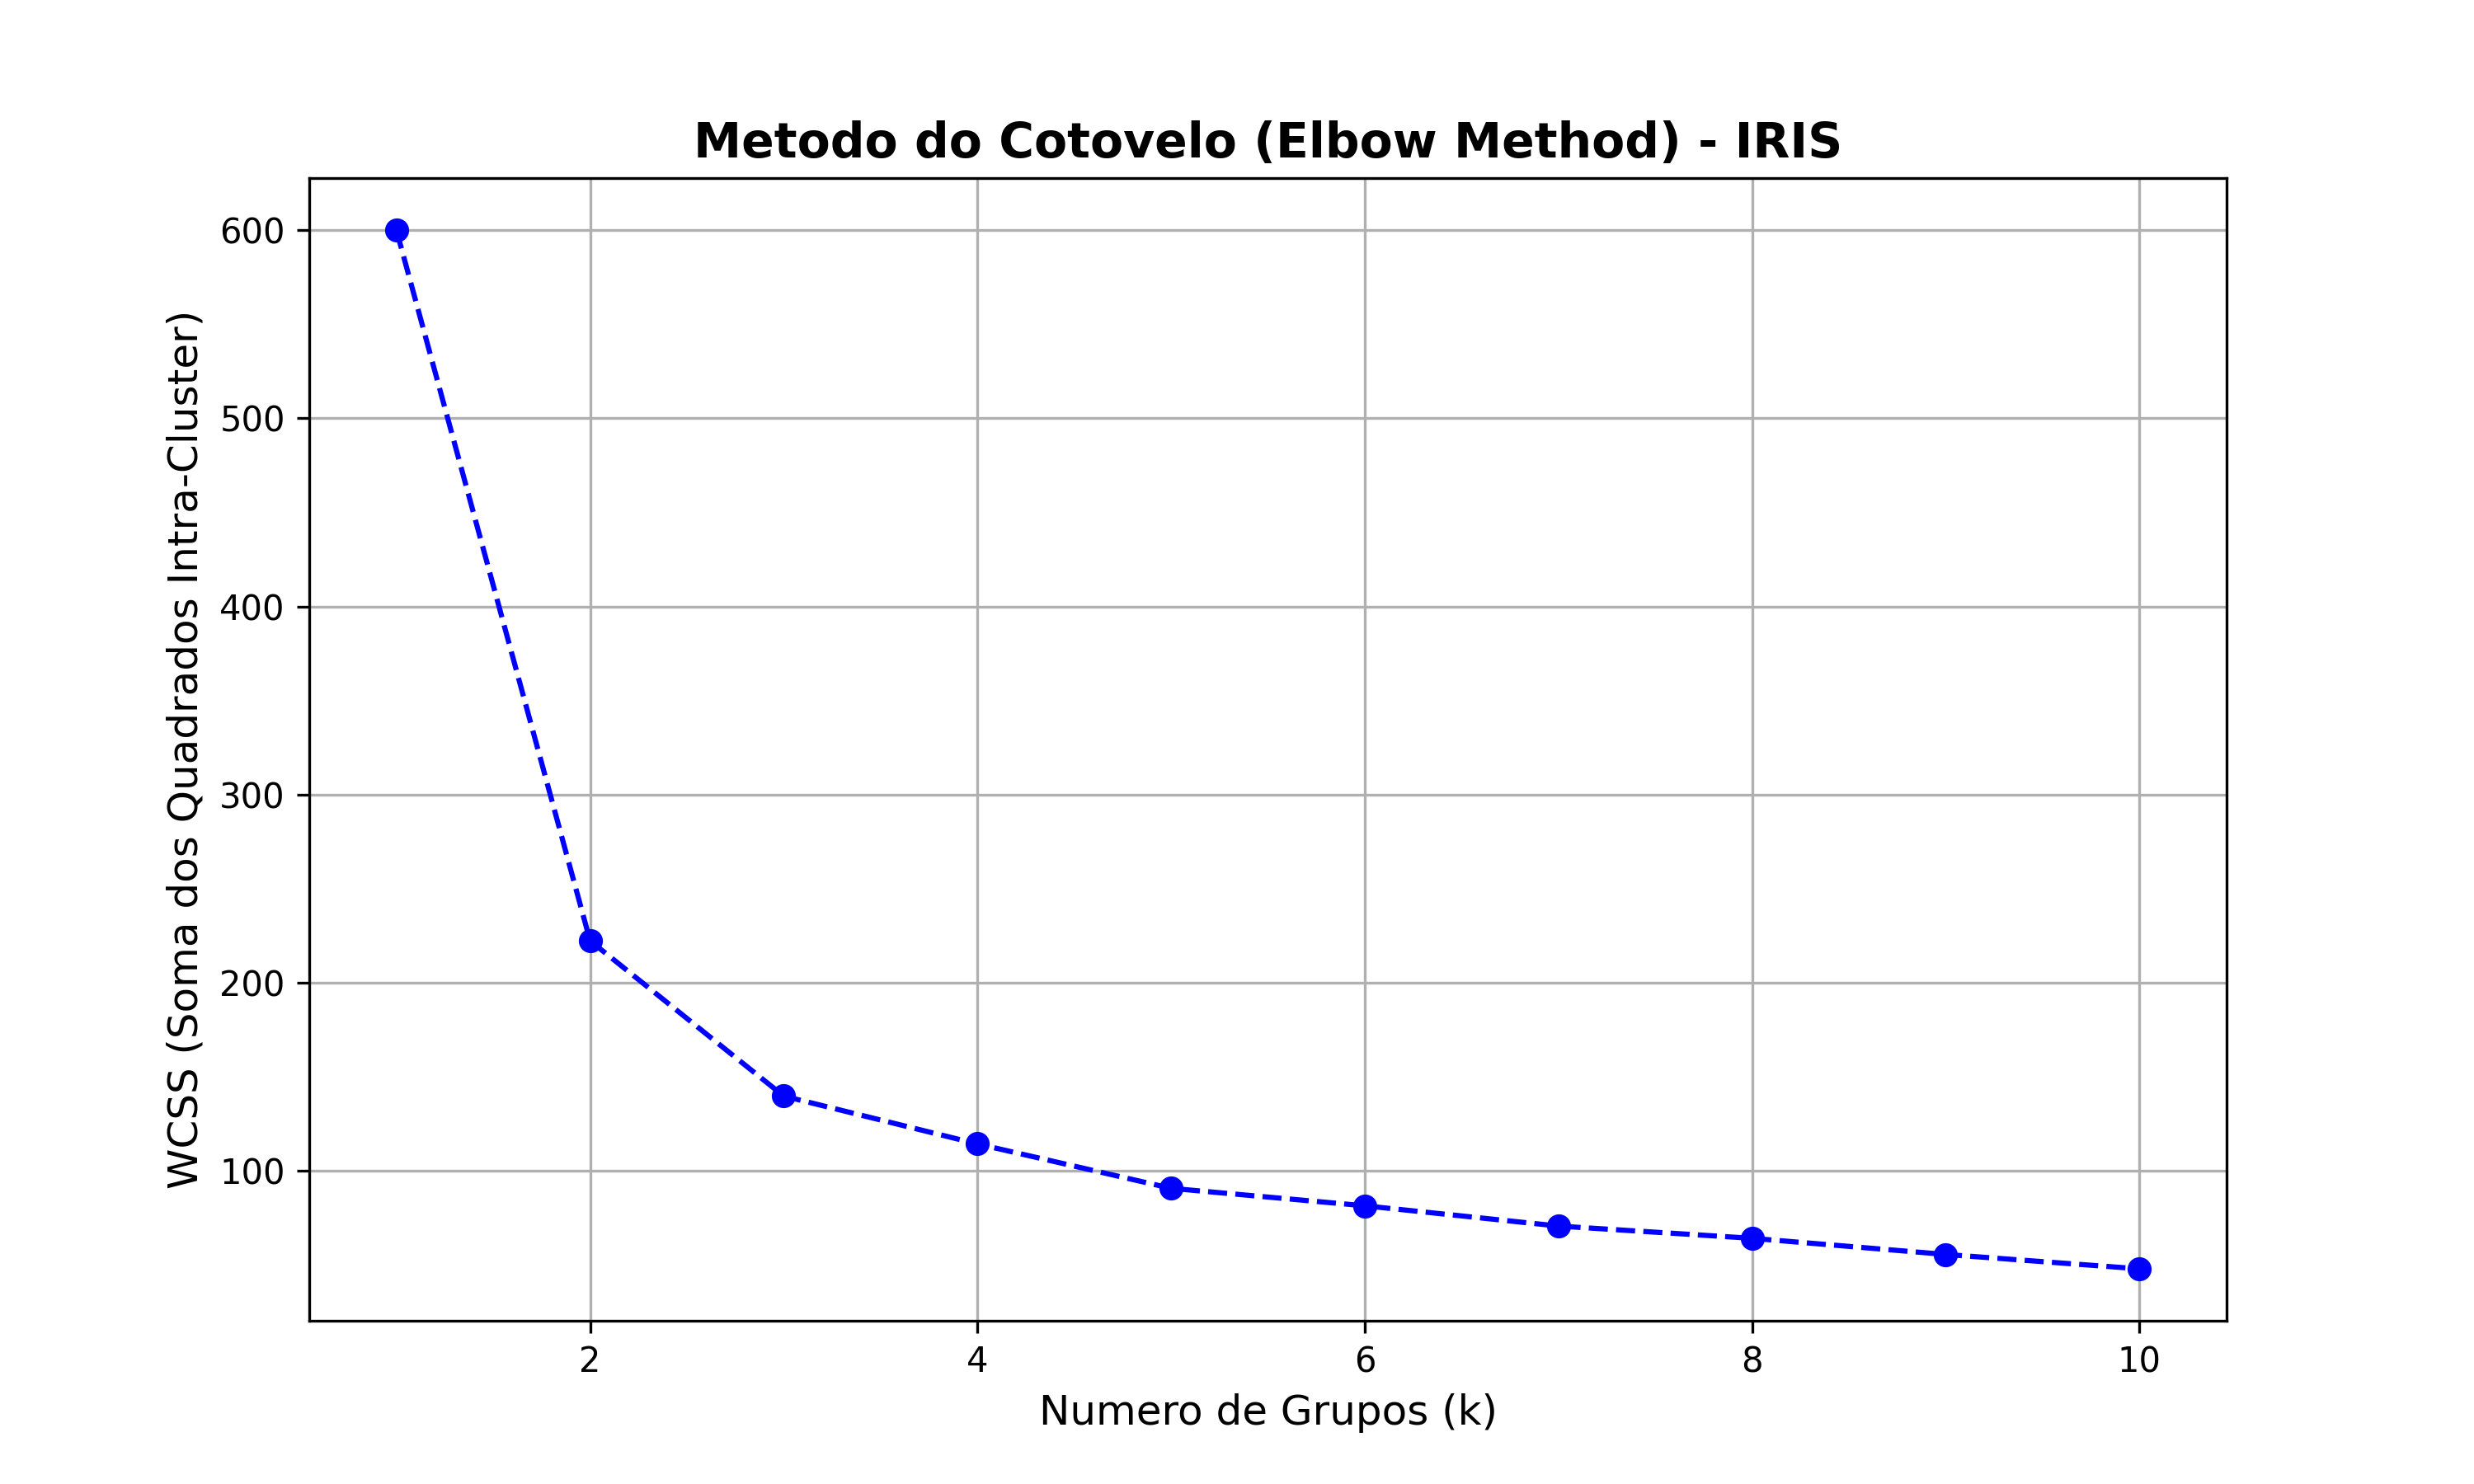
\includegraphics[width=.9\linewidth]{figures/kmeans_elbow_iris.png}
\caption{Analise do Metodo do Cotovelo}
\end{figure}

\begin{figure}[htbp]
\centering
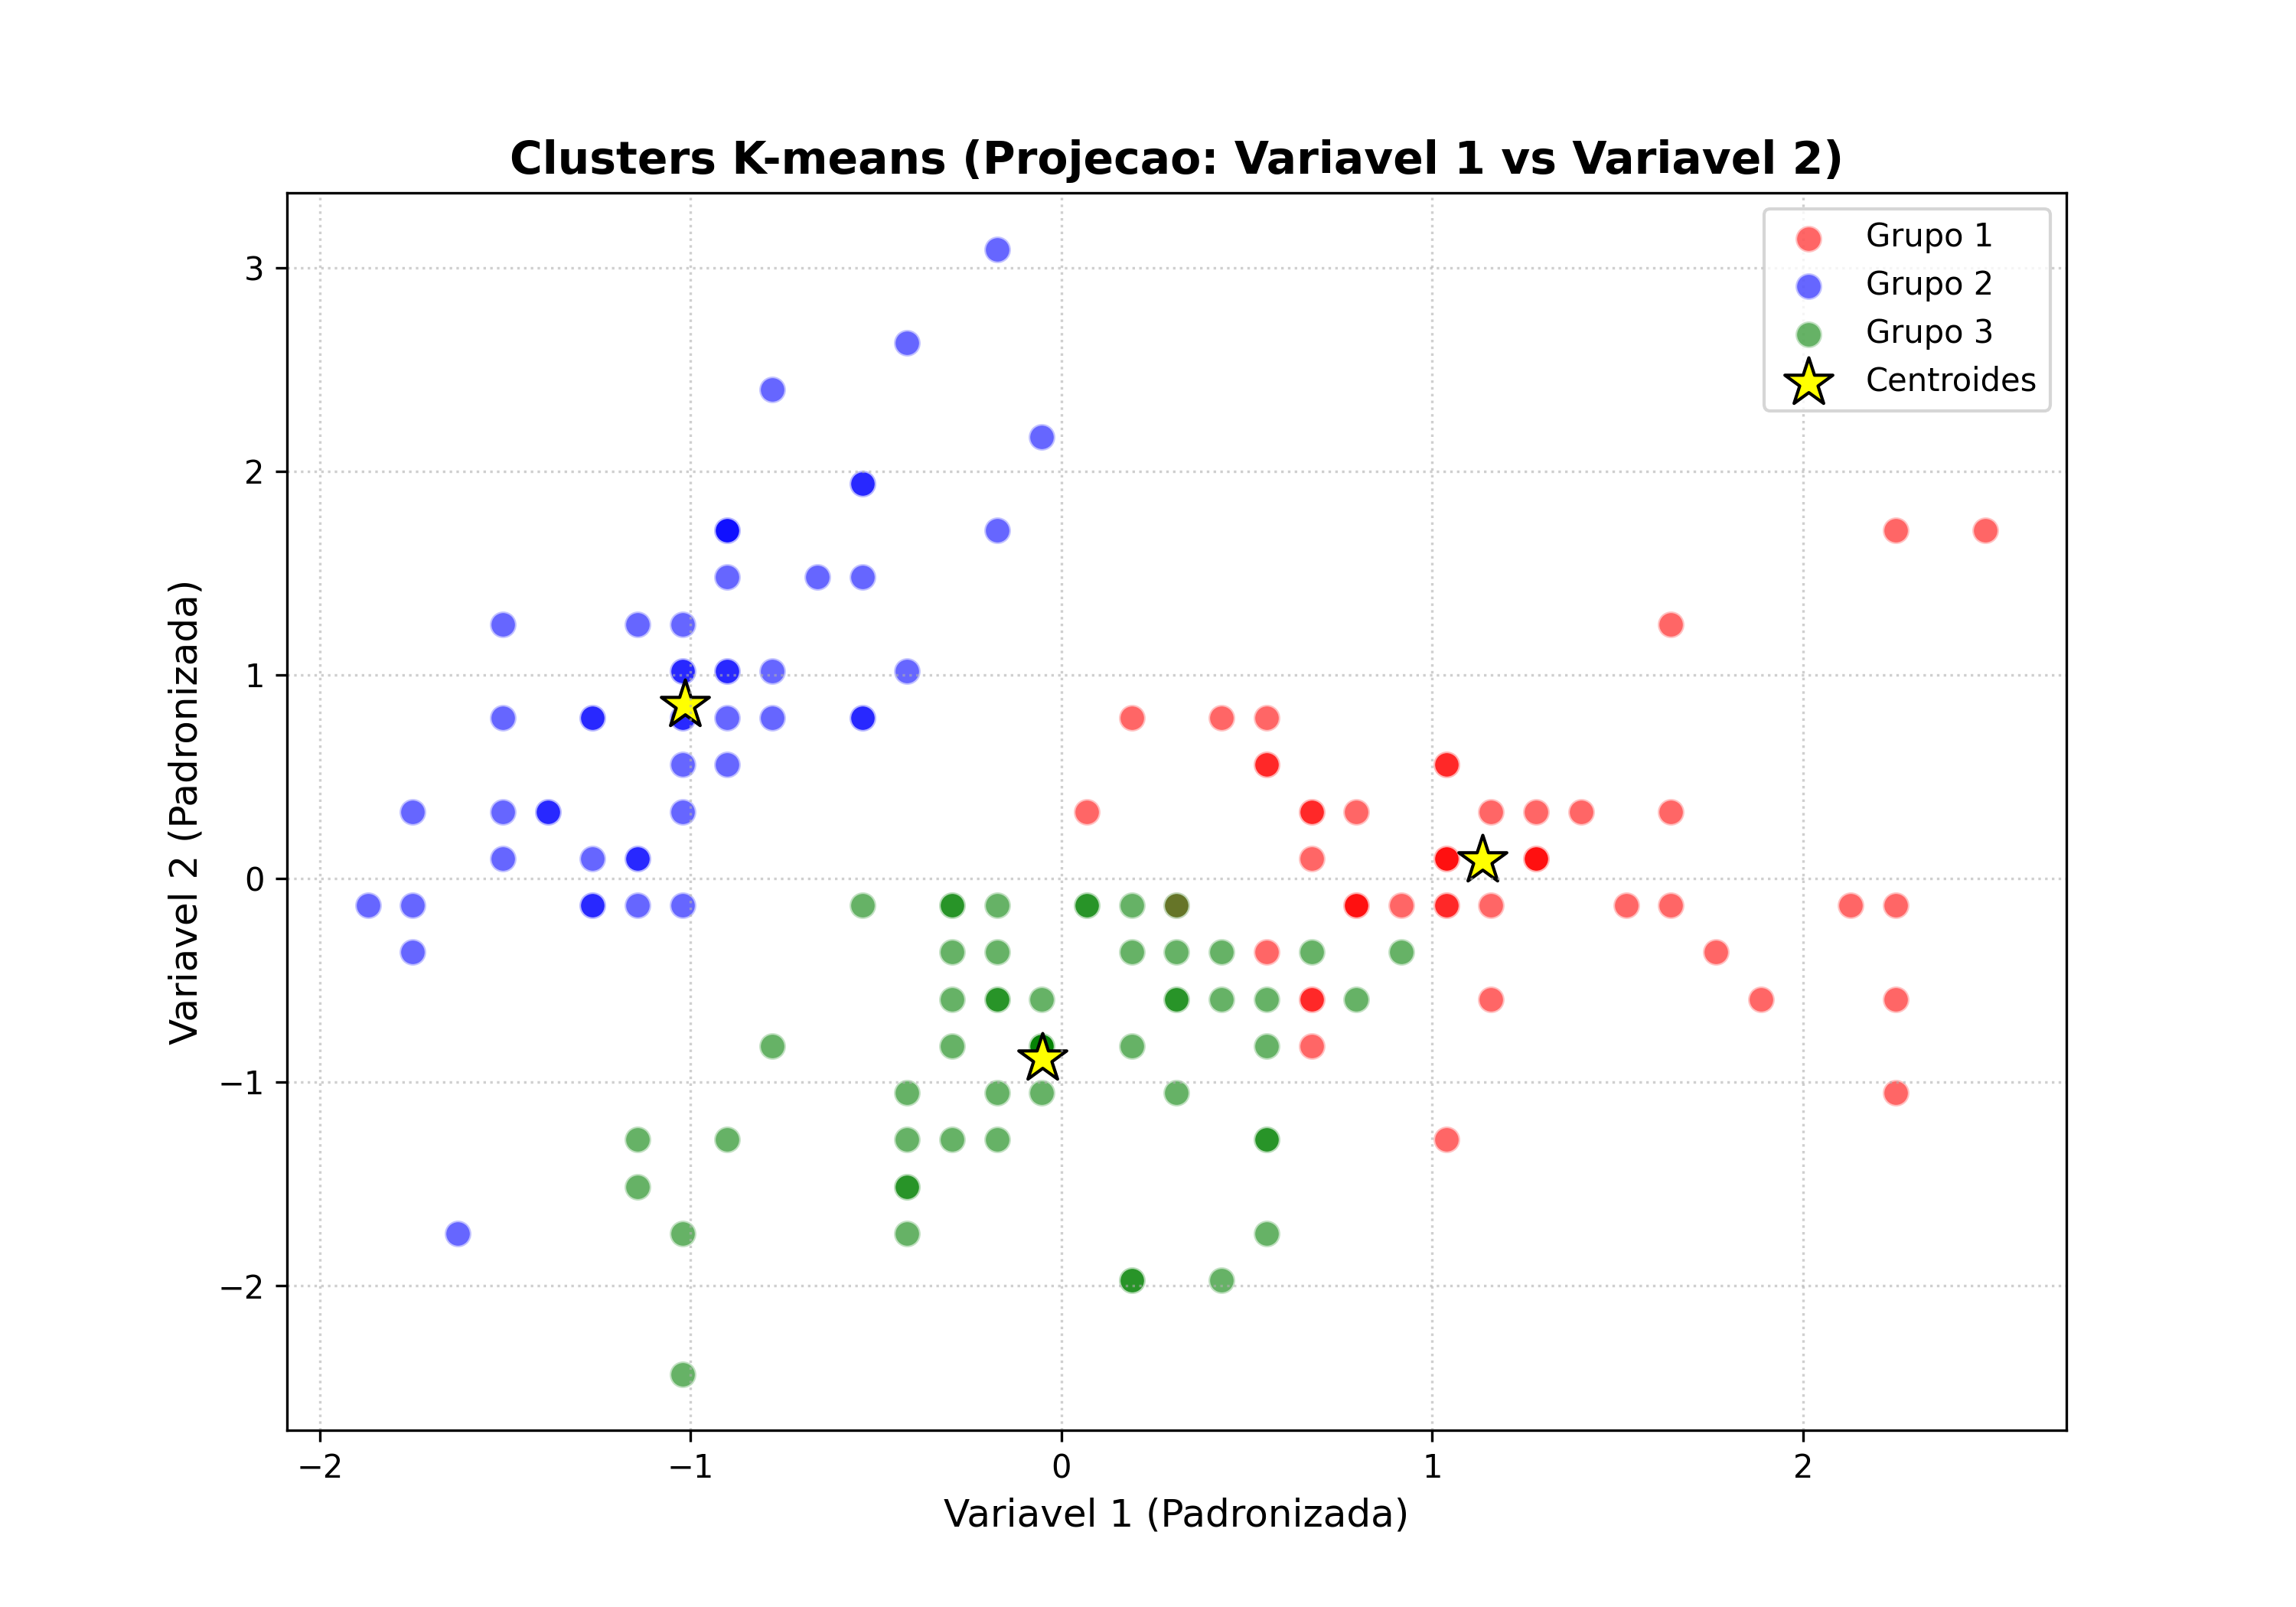
\includegraphics[width=.9\linewidth]{figures/kmeans_scatter_iris.png}
\caption{Dispersao dos Grupos (Cotovelo)}
\end{figure}
\subsection{Abordagem 2: K-means Simples com Validacao Estatistica}
\label{sec:org31ba52c}
Nesta versao, definimos o numero de grupos diretamente e realizamos testes de ANOVA e MANOVA para verificar se os grupos sao estatisticamente distintos.

\begin{verbatim}
# %%
import ex2_1_load_iris
import ex2_2_clustering_iris
import pandas as pd
import numpy as np
from sklearn.preprocessing import StandardScaler

# 1. Leitura dos dados
df = ex2_1_load_iris.load_iris_data()


# 2. Mostrar as primeiras 10 linhas
print("--- Primeiras 10 linhas do dataset IRIS ---")
print(df.head(10))

# 3. Padronizacao (Escalonamento)
# Selecionamos as colunas numericas (SEPALLEN, SEPALWID, PETALLEN, PETALWID)
variaveis_list = ['SEPALLEN', 'SEPALWID', 'PETALLEN', 'PETALWID']
mtz_vlrs = df[variaveis_list].values
species = df['specie'].values

scaler = StandardScaler()
mtz_vlrs_padrozinados = scaler.fit_transform(mtz_vlrs)

print("\nDados padronizados (primeiras 5 linhas):")
print(mtz_vlrs_padrozinados[:5])

# 4. Definicao do numero de grupos
# Altere este valor para escolher quantos grupos deseja formar
n_grupos = 3

# 5. Executar K-means
print(f"\n--- Executando K-means (k={n_grupos}) ---")
df_grupos, kmeans_model = ex2_2_clustering_iris.executar_kmeans(
    mtz_vlrs_padrozinados, 
    species, 
    n_clusters=n_grupos
)

# Adicionando a informacao do grupo ao DataFrame original
df['Grupo'] = df_grupos['Grupo']

# 6. Mostrar resultados
print("\n--- Dados Originais com Atribuicao de Grupos (K-means) ---")
print(df.head(10))

# Verificar a contagem em cada grupo
print("\nContagem por grupo:")
print(df_grupos['Grupo'].value_counts())
print(df['Grupo'].value_counts())

# exibir nome das variaveis e os grupos atribuídos em df
print("\n--- Variaveis e Grupos Atribuidos ---")


# Comparar com as especies originais (Crosstab)
print("\n--- Cruzamento: Especie Original vs Grupo K-means ---")
print(pd.crosstab(df['specie'], df['Grupo']))


# 7. Visualizacao dos clusters
print("\n--- Gerando Grafico de Dispersao dos Clusters ---")
ex2_2_clustering_iris.plot_kmeans_clusters(
    mtz_vlrs_padrozinados, 
    df_grupos['Grupo'].values, 
    kmeans_model.cluster_centers_,
    filename='kmeans_scatter_iris_simple.png'
)

# 8. Analise Univariada (ANOVA) - Verificando a qualidade dos grupos
#  1. Iteração por Variável: Para cada uma das 4 variáveis (SEPALLEN, SEPALWID, etc.), ele realiza um teste ANOVA.
#   2. Teste de Hipótese:
#       * H0 (Hipótese Nula): As médias de todos os grupos são iguais para aquela variável (o agrupamento não foi eficaz para distinguir essa característica).
#       * H1 (Hipótese Alternativa): Pelo menos um grupo tem uma média significativamente diferente (o agrupamento conseguiu separar bem essa característica).
#   O script já interpreta o p-valor (usando o padrão de 5% ou 0.05) e te diz se o resultado foi significativo.
#
#  Se os grupos forem bons, esperamos que o p-valor seja muito pequeno (ex: algo como 1.23e-15) e a mensagem diga "Significativo" para a maioria das variáveis.
#
#  Pode rodar o script novamente para ver os resultados:
import statsmodels.api as sm
from statsmodels.formula.api import ols

print("\n--- Analise de Variancia (ANOVA) por Variavel ---")
print("H0: Nao ha diferenca entre as medias dos grupos")
print("H1: Ha pelo menos uma diferenca entre as medias")

for var in variaveis_list:
    formula = f"{var} ~ C(Grupo)"
    model = ols(formula, data=df).fit()
    anova_table = sm.stats.anova_lm(model, typ=2)
    
    # Acessando os valores usando o nome da linha 'C(Grupo)'
    p_valor = anova_table.at['C(Grupo)', 'PR(>F)']
    f_stat = anova_table.at['C(Grupo)', 'F']
    
    print(f"\nVariavel: {var}")
    print(f"F-statistic: {f_stat:.4f}")
    print(f"p-valor: {p_valor:.4e}")
    
    if p_valor < 0.05:
        print("Resultado: Significativo (Existem diferencas entre os grupos)")
    else:
        print("Resultado: Nao significativo (Nao ha diferencas claras)")

# 9. Analise Multivariada de Variancia (MANOVA)
from statsmodels.multivariate.manova import MANOVA

print("\n--- Analise Multivariada de Variancia (MANOVA) ---")
print("H0: Os vetores de medias dos grupos sao iguais")
print("H1: Pelo menos um vetor de media e diferente")

# Criando a formula para todas as variaveis dependentes
# Ex: "SEPALLEN + SEPALWID + PETALLEN + PETALWID ~ C(Grupo)"
formula_manova = " + ".join(variaveis_list) + " ~ C(Grupo)"
manova = MANOVA.from_formula(formula_manova, data=df)

# Exibindo os resultados (Wilks' lambda, Pillai's trace, etc)
print(manova.mv_test())

#from notebooklm
#referencias do livro Hair et al. (2024) para interpretação dos resultados da MANOVA:
#Aqui está como o livro orienta a interpretação de cada uma dessas quatro medidas estatísticas:
#Lambda de Wilks (Wilks' lambda): É a estatística mais comumente utilizada para testar a significância geral entre os grupos. Ela considera todas as funções discriminantes para examinar se os grupos são de algum modo diferentes[fn:760].
#Critério de Pillai (Pillai's trace) e Traço de Hotelling (Hotelling-Lawley trace): São medidas semelhantes ao Lambda de Wilks, pois também consideram todas as raízes características (ou seja, avaliam todas as dimensões de diferença simultaneamente)[fn:760].
#Maior raiz característica de Roy (Roy's greatest root): Diferentemente das outras três, esta estatística mede as diferenças focando apenas na primeira função discriminante (a dimensão principal)[fn:517][fn:760].
##Como o livro recomenda escolher entre elas? Apesar de, na grande maioria das vezes, todas levarem à mesma conclusão, Hair et al. apontam diretrizes específicas para a escolha do melhor indicador, dependendo das características dos seus dados[fn:761]:
#Critério de Pillai: É considerado o teste mais robusto. O autor recomenda que ele seja utilizado (junto ou no lugar do Lambda de Wilks) caso ocorram violações nas suposições básicas: se o tamanho da amostra diminuir, se os grupos tiverem tamanhos muito diferentes (células desiguais), ou se a suposição de homogeneidade de covariâncias for violada[fn:761].
#Lambda de Wilks ou Pillai: São as medidas de preferência quando as considerações básicas de planejamento foram atendidas perfeitamente (amostra adequada, pressupostos atendidos e células proporcionais)[fn:761].
#Maior Raiz de Roy: É o teste estatístico mais poderoso, mas apenas se o pesquisador estiver seguro de que todas as suposições (como normalidade e homocedasticidade) foram estritamente cumpridas e que as variáveis dependentes estão fortemente inter-relacionadas em uma única dimensão de efeito[fn:760][fn:761].
#Interpretando o seu resultado específico: Observando a sua tabela na seção C(Grupo), a coluna Pr > F (que é o seu p-valor) apresenta 0.0000 para todos os quatro testes.
##A interpretação prática usando as diretrizes do Hair é que, independentemente do critério utilizado — seja o mais poderoso (Roy) ou o mais robusto (Pillai) —, existe uma diferença estatisticamente altamente significativa entre os seus grupos. O modelo demonstra que o fator Grupo afeta as variáveis analisadas de forma conjunta, com uma probabilidade de isso ser obra do acaso praticamente nula.
#Referências [fn:517] Hair et al., Análise Multivariada de Dados (Significância geral - Estimação simultânea em Análise Discriminante). [fn:760] Hair et al., Análise Multivariada de Dados (Medidas estatísticas para avaliação de diferenças ao longo de dimensões - MANOVA). [fn:761] Hair et al., Análise Multivariada de Dados (Diretrizes e robustez dos testes Wilks, Pillai, Hotelling e Roy).
\end{verbatim}
\captionof{figure}{Script K-means Simples e Validacao}
\subsubsection{Analise de Resultados}
\label{sec:org9e5ef22}
A analise inclui:
\begin{itemize}
\item \textbf{Crosstab}: Comparacao entre a especie real e o grupo atribuido.
\item \textbf{ANOVA}: Teste univariado para cada variavel (SEPALLEN, SEPALWID, etc).
\item \textbf{MANOVA}: Teste multivariado considerando todas as variaveis simultaneamente.
\end{itemize}

\begin{figure}[htbp]
\centering
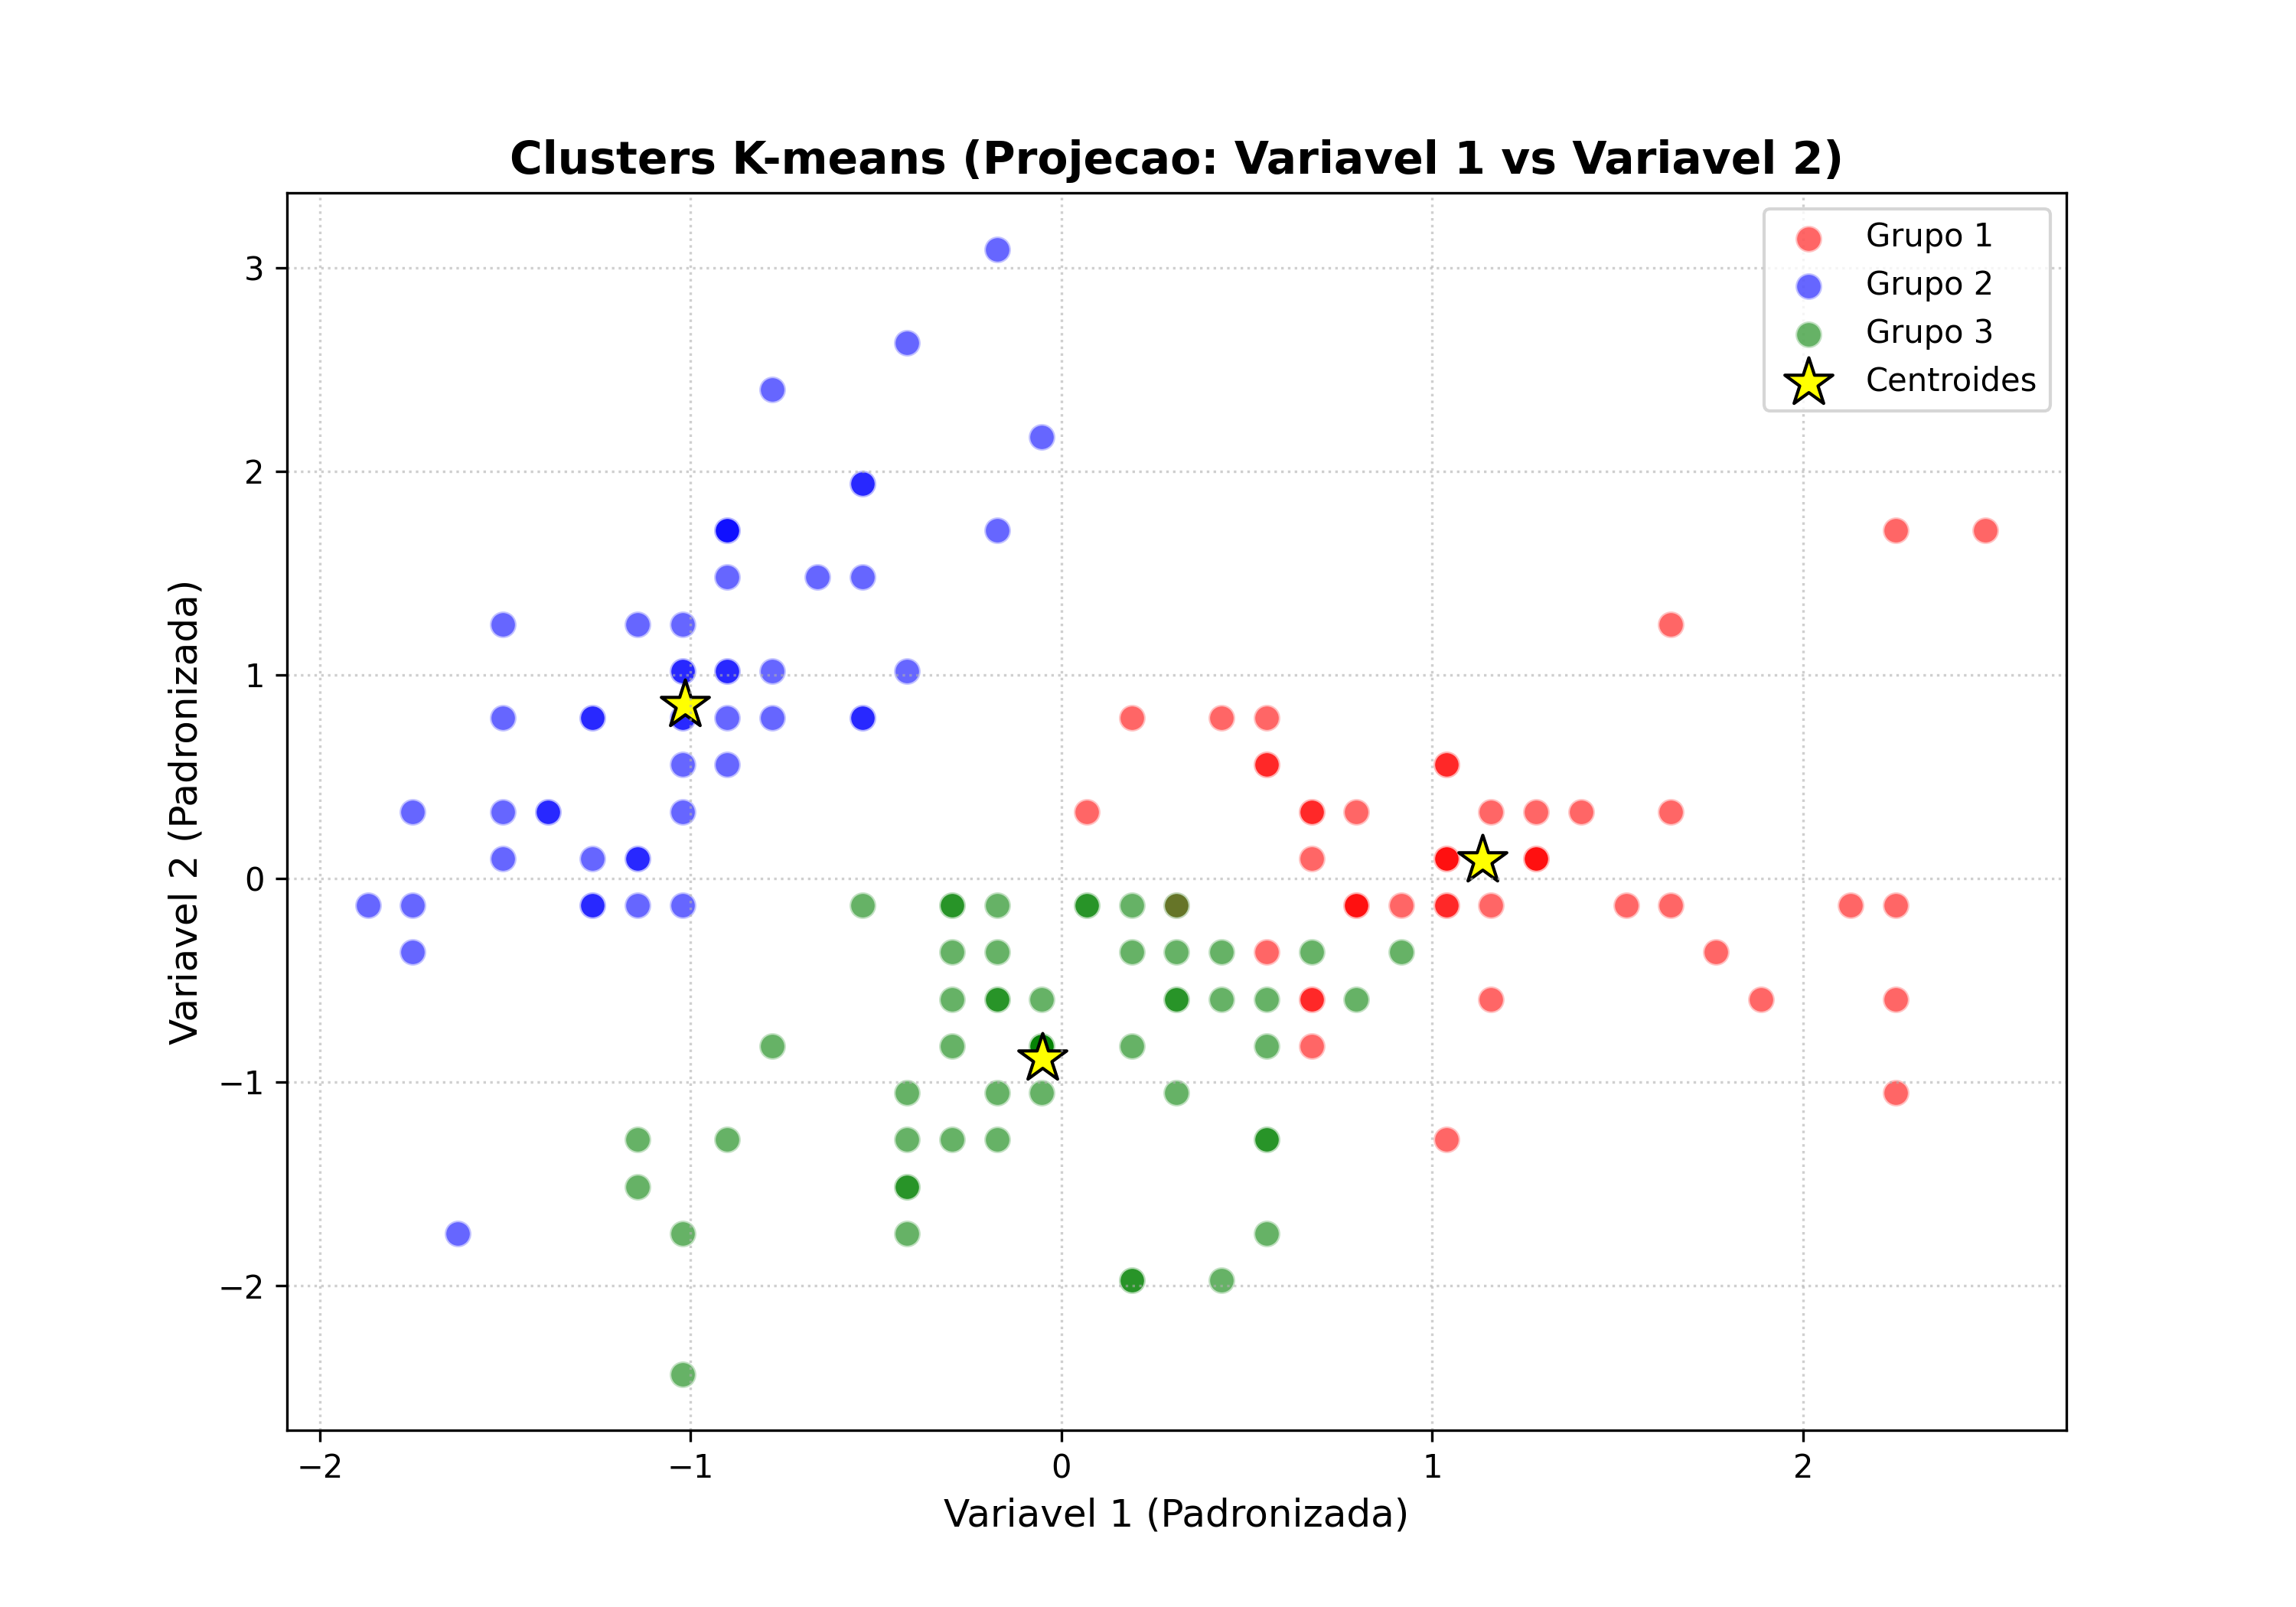
\includegraphics[width=.9\linewidth]{figures/kmeans_scatter_iris_simple.png}
\caption{Dispersao dos Grupos (Simples)}
\end{figure}
\section{Conclusao}
\label{sec:org57433a2}

Consegui praticar a análise de agrupamento

O Livro do hair não fala do método ebowl de kmeans mas percebi que as
multiplos agrupamentos me pareceu resultar em grupos melhores que no
kmeans simples onde eu escolhi 3 grupos e os grupos foram formados sem
a inteligencia do ebowl.
Já o dendograma é uma técnica mais interessante porque podemos
escolher o ponto de corte. Consegui colocar isso no código, podemos
cortar e obter os grupos.
Agradeço muitíssimo a oportunidade e a compreenção.
\section{saida completo do ex1 dendograma}
\label{sec:org67c6e93}

\begin{verbatim}
(venv) wgn@fedora:~/WORKING/Projects-Srcs/Projects-Srcs-FzlSoft/curso_estatistica_multivariada$ python3 exercicios/exercicio_1/src/main_ex1.py 
--- Primeiras 10 linhas do dataframe ---
  species  loc_1  loc_2  loc_3  loc_4  loc_5  loc_6  loc_7  loc_8  loc_9  loc_10  ...  loc_20  loc_21  loc_22  loc_23  loc_24  loc_25  loc_26  loc_27  loc_28  loc_29  loc_30
0   esp_1      0      0      1      1      0      1      1      0      0       0  ...       1       0       1       0       0       0       1       1       1       0       0
1   esp_2      0      0      1      0      1      0      0      0      1       1  ...       0       0       1       0       0       0       1       0       1       0       0
2   esp_3      0      0      1      0      1      0      0      0      1       1  ...       0       0       1       0       0       1       1       0       1       0       0
3   esp_4      0      0      1      1      0      0      0      0      1       1  ...       0       0       1       0       0       0       1       0       1       0       1
4   esp_5      0      0      1      0      1      0      0      0      1       1  ...       0       0       1       0       0       1       0       0       1       0       0
5   esp_6      1      0      0      0      0      0      1      1      0       0  ...       1       1       1       1       0       0       0       0       0       1       1
6   esp_7      0      0      1      1      1      0      1      0      1       0  ...       0       0       1       1       1       1       0       1       0       0       1
7   esp_8      1      0      0      0      0      1      1      0      1       1  ...       0       1       0       1       0       1       1       0       1       0       0

[8 rows x 31 columns]

--- Matriz de Distancia (Sorensen-Dice) ---
       esp_1  esp_2  esp_3  esp_4  esp_5  esp_6  esp_7  esp_8
esp_1  0.000  0.478  0.500  0.360  0.565  0.680  0.429  0.615
esp_2  0.478  0.000  0.053  0.200  0.111  0.900  0.565  0.524
esp_3  0.500  0.053  0.000  0.238  0.053  0.905  0.500  0.455
esp_4  0.360  0.200  0.238  0.000  0.300  0.818  0.520  0.565
esp_5  0.565  0.111  0.053  0.300  0.000  0.900  0.478  0.524
esp_6  0.680  0.900  0.905  0.818  0.900  0.000  0.600  0.652
esp_7  0.429  0.565  0.500  0.520  0.478  0.600  0.000  0.615
esp_8  0.615  0.524  0.455  0.565  0.524  0.652  0.615  0.000

--- Matriz de Distancia (Simple Matching) ---
       esp_1  esp_2  esp_3  esp_4  esp_5  esp_6  esp_7  esp_8
esp_1  0.000  0.367  0.400  0.300  0.433  0.567  0.400  0.533
esp_2  0.367  0.000  0.033  0.133  0.067  0.600  0.433  0.367
esp_3  0.400  0.033  0.000  0.167  0.033  0.633  0.400  0.333
esp_4  0.300  0.133  0.167  0.000  0.200  0.600  0.433  0.433
esp_5  0.433  0.067  0.033  0.200  0.000  0.600  0.367  0.367
esp_6  0.567  0.600  0.633  0.600  0.600  0.000  0.500  0.500
esp_7  0.400  0.433  0.400  0.433  0.367  0.500  0.000  0.533
esp_8  0.533  0.367  0.333  0.433  0.367  0.500  0.533  0.000

--- Gerando Dendrogramas ---
Dendrograma salvo em: /home/wgn/WORKING/Projects-Srcs/Projects-Srcs-FzlSoft/curso_estatistica_multivariada/exercicios/exercicio_1/src/../text/figures/dendrograma_sorensen_dice.png
Dendrograma salvo em: /home/wgn/WORKING/Projects-Srcs/Projects-Srcs-FzlSoft/curso_estatistica_multivariada/exercicios/exercicio_1/src/../text/figures/dendrograma_simple_matching.png

--- Atribuicao de Grupos (Exemplos) ---

Grupos (Sorensen-Dice, k=3):
  Especie  Grupo
0   esp_1      1
1   esp_2      1
2   esp_3      1
3   esp_4      1
4   esp_5      1
5   esp_6      3
6   esp_7      1
7   esp_8      2

Grupos (Simple Matching, h=0.4):
  Especie  Grupo
0   esp_1      1
1   esp_2      1
2   esp_3      1
3   esp_4      1
4   esp_5      1
5   esp_6      4
6   esp_7      2
7   esp_8      3
(venv)
  wgn@fedora:~/WORKING/Projects-Srcs/Projects-Srcs-FzlSoft/curso_estatistica_multivariada$
\end{verbatim}
\section{saida completa do kmeans simples}
\label{sec:org0bd9166}

\begin{verbatim}
  (venv) wgn@fedora:~/WORKING/Projects-Srcs/Projects-Srcs-FzlSoft/curso_estatistica_multivariada$ python3 exercicios/exercicio_1/src/main_ex2_kmeans_simple.py 
--- Primeiras 10 linhas do dataset IRIS ---
     specie  SEPALLEN  SEPALWID  PETALLEN  PETALWID
0    SETOSA       5.0       3.3       1.4       0.2
1  VIRGINIC       6.4       2.8       5.6       2.2
2  VERSICOL       6.5       2.8       4.6       1.5
3  VIRGINIC       6.7       3.1       5.6       2.4
4  VIRGINIC       6.3       2.8       5.1       1.5
5    SETOSA       4.6       3.4       1.4       0.3
6  VIRGINIC       6.9       3.1       5.1       2.3
7  VERSICOL       6.2       2.2       4.5       1.5
8  VERSICOL       5.9       3.2       4.8       1.8
9    SETOSA       4.6       3.6       1.0       0.2

Dados padronizados (primeiras 5 linhas):
[[-1.02184904  0.55861082 -1.34022653 -1.3154443 ]
 [ 0.67450115 -0.59237301  1.0469454   1.31719939]
 [ 0.79566902 -0.59237301  0.47857113  0.3957741 ]
 [ 1.03800476  0.09821729  1.0469454   1.58046376]
 [ 0.55333328 -0.59237301  0.76275827  0.3957741 ]]

--- Executando K-means (k=3) ---

--- Dados Originais com Atribuicao de Grupos (K-means) ---
     specie  SEPALLEN  SEPALWID  PETALLEN  PETALWID  Grupo
0    SETOSA       5.0       3.3       1.4       0.2      2
1  VIRGINIC       6.4       2.8       5.6       2.2      1
2  VERSICOL       6.5       2.8       4.6       1.5      3
3  VIRGINIC       6.7       3.1       5.6       2.4      1
4  VIRGINIC       6.3       2.8       5.1       1.5      3
5    SETOSA       4.6       3.4       1.4       0.3      2
6  VIRGINIC       6.9       3.1       5.1       2.3      1
7  VERSICOL       6.2       2.2       4.5       1.5      3
8  VERSICOL       5.9       3.2       4.8       1.8      1
9    SETOSA       4.6       3.6       1.0       0.2      2

Contagem por grupo:
Grupo
3    53
2    50
1    47
Name: count, dtype: int64
Grupo
3    53
2    50
1    47
Name: count, dtype: int64

--- Variaveis e Grupos Atribuidos ---

--- Cruzamento: Especie Original vs Grupo K-means ---
Grupo      1   2   3
specie              
SETOSA     0  50   0
VERSICOL  11   0  39
VIRGINIC  36   0  14

--- Gerando Grafico de Dispersao dos Clusters ---
Grafico de Clusters (Scatter) salvo em: /home/wgn/WORKING/Projects-Srcs/Projects-Srcs-FzlSoft/curso_estatistica_multivariada/exercicios/exercicio_1/src/../text/figures/kmeans_scatter_iris_simple.png

--- Analise de Variancia (ANOVA) por Variavel ---
H0: Nao ha diferenca entre as medias dos grupos
H1: Ha pelo menos uma diferenca entre as medias

Variavel: SEPALLEN
F-statistic: 218.5710
p-valor: 9.0932e-45
Resultado: Significativo (Existem diferencas entre os grupos)

Variavel: SEPALWID
F-statistic: 79.9000
p-valor: 3.2655e-24
Resultado: Significativo (Existem diferencas entre os grupos)

Variavel: PETALLEN
F-statistic: 860.6367
p-valor: 7.0300e-82
Resultado: Significativo (Existem diferencas entre os grupos)

Variavel: PETALWID
F-statistic: 525.6988
p-valor: 1.0487e-67
Resultado: Significativo (Existem diferencas entre os grupos)

--- Analise Multivariada de Variancia (MANOVA) ---
H0: Os vetores de medias dos grupos sao iguais
H1: Pelo menos um vetor de media e diferente
                   Multivariate linear model
================================================================
                                                                
----------------------------------------------------------------
       Intercept         Value  Num DF  Den DF   F Value  Pr > F
----------------------------------------------------------------
          Wilks' lambda  0.0104 4.0000 144.0000 3416.6552 0.0000
         Pillai's trace  0.9896 4.0000 144.0000 3416.6552 0.0000
 Hotelling-Lawley trace 94.9071 4.0000 144.0000 3416.6552 0.0000
    Roy's greatest root 94.9071 4.0000 144.0000 3416.6552 0.0000
----------------------------------------------------------------
                                                                
----------------------------------------------------------------
         C(Grupo)         Value  Num DF  Den DF  F Value  Pr > F
----------------------------------------------------------------
           Wilks' lambda  0.0383 8.0000 288.0000 148.0632 0.0000
          Pillai's trace  1.3728 8.0000 290.0000  79.3376 0.0000
  Hotelling-Lawley trace 14.3967 8.0000 203.4024 258.0786 0.0000
     Roy's greatest root 13.6070 4.0000 145.0000 493.2547 0.0000
================================================================

(venv) wgn@fedora:~/WORKING/Projects-Srcs/Projects-Srcs-FzlSoft/curso_estatistica_multivariada$ 

\end{verbatim}
\section{saída completa do kmeans com ebowol}
\label{sec:org12e43fb}

\begin{verbatim}
(venv) wgn@fedora:~/WORKING/Projects-Srcs/Projects-Srcs-FzlSoft/curso_estatistica_multivariada$ python3 exercicios/exercicio_1/src/main_ex2_kmeans_elbow.py 
--- Primeiras 10 linhas do dataset IRIS ---
     specie  SEPALLEN  SEPALWID  PETALLEN  PETALWID
0    SETOSA       5.0       3.3       1.4       0.2
1  VIRGINIC       6.4       2.8       5.6       2.2
2  VERSICOL       6.5       2.8       4.6       1.5
3  VIRGINIC       6.7       3.1       5.6       2.4
4  VIRGINIC       6.3       2.8       5.1       1.5
5    SETOSA       4.6       3.4       1.4       0.3
6  VIRGINIC       6.9       3.1       5.1       2.3
7  VERSICOL       6.2       2.2       4.5       1.5
8  VERSICOL       5.9       3.2       4.8       1.8
9    SETOSA       4.6       3.6       1.0       0.2

Dados padronizados (primeiras 5 linhas):
[[-1.02184904  0.55861082 -1.34022653 -1.3154443 ]
 [ 0.67450115 -0.59237301  1.0469454   1.31719939]
 [ 0.79566902 -0.59237301  0.47857113  0.3957741 ]
 [ 1.03800476  0.09821729  1.0469454   1.58046376]
 [ 0.55333328 -0.59237301  0.76275827  0.3957741 ]]

--- Analise do Numero Otimo de Grupos (Metodo do Cotovelo) ---
Grafico do Cotovelo salvo em: /home/wgn/WORKING/Projects-Srcs/Projects-Srcs-FzlSoft/curso_estatistica_multivariada/exercicios/exercicio_1/src/../text/figures/kmeans_elbow_iris.png

--- Executando K-means (k=3) ---

--- Dados Originais com Atribuicao de Grupos (K-means) ---
     specie  SEPALLEN  SEPALWID  PETALLEN  PETALWID  Grupo
0    SETOSA       5.0       3.3       1.4       0.2      2
1  VIRGINIC       6.4       2.8       5.6       2.2      1
2  VERSICOL       6.5       2.8       4.6       1.5      3
3  VIRGINIC       6.7       3.1       5.6       2.4      1
4  VIRGINIC       6.3       2.8       5.1       1.5      3
5    SETOSA       4.6       3.4       1.4       0.3      2
6  VIRGINIC       6.9       3.1       5.1       2.3      1
7  VERSICOL       6.2       2.2       4.5       1.5      3
8  VERSICOL       5.9       3.2       4.8       1.8      1
9    SETOSA       4.6       3.6       1.0       0.2      2

Contagem por grupo:
Grupo
3    53
2    50
1    47
Name: count, dtype: int64

--- Cruzamento: Especie Original vs Grupo K-means ---
Grupo      1   2   3
specie              
SETOSA     0  50   0
VERSICOL  11   0  39
VIRGINIC  36   0  14

--- Gerando Grafico de Dispersao dos Clusters ---
Grafico de Clusters (Scatter) salvo em: /home/wgn/WORKING/Projects-Srcs/Projects-Srcs-FzlSoft/curso_estatistica_multivariada/exercicios/exercicio_1/src/../text/figures/kmeans_scatter_iris.png

--- Analise de Variancia (ANOVA) por Variavel ---
H0: Nao ha diferenca entre as medias dos grupos
H1: Ha pelo menos uma diferenca entre as medias

Variavel: SEPALLEN
F-statistic: 218.5710
p-valor: 9.0932e-45
Resultado: Significativo (Existem diferencas entre os grupos)

Variavel: SEPALWID
F-statistic: 79.9000
p-valor: 3.2655e-24
Resultado: Significativo (Existem diferencas entre os grupos)

Variavel: PETALLEN
F-statistic: 860.6367
p-valor: 7.0300e-82
Resultado: Significativo (Existem diferencas entre os grupos)

Variavel: PETALWID
F-statistic: 525.6988
p-valor: 1.0487e-67
Resultado: Significativo (Existem diferencas entre os grupos)

--- Analise Multivariada de Variancia (MANOVA) ---
H0: Os vetores de medias dos grupos sao iguais
H1: Pelo menos um vetor de media e diferente
                   Multivariate linear model
================================================================
                                                                
----------------------------------------------------------------
       Intercept         Value  Num DF  Den DF   F Value  Pr > F
----------------------------------------------------------------
          Wilks' lambda  0.0104 4.0000 144.0000 3416.6552 0.0000
         Pillai's trace  0.9896 4.0000 144.0000 3416.6552 0.0000
 Hotelling-Lawley trace 94.9071 4.0000 144.0000 3416.6552 0.0000
    Roy's greatest root 94.9071 4.0000 144.0000 3416.6552 0.0000
----------------------------------------------------------------
                                                                
----------------------------------------------------------------
         C(Grupo)         Value  Num DF  Den DF  F Value  Pr > F
----------------------------------------------------------------
           Wilks' lambda  0.0383 8.0000 288.0000 148.0632 0.0000
          Pillai's trace  1.3728 8.0000 290.0000  79.3376 0.0000
  Hotelling-Lawley trace 14.3967 8.0000 203.4024 258.0786 0.0000
     Roy's greatest root 13.6070 4.0000 145.0000 493.2547 0.0000
================================================================

(venv) wgn@fedora:~/WORKING/Projects-Srcs/Projects-Srcs-FzlSoft/curso_estatistica_multivariada$ 
\end{verbatim}
\end{document}
